%\documentclass{sig-alternate}
\documentclass{sig-alt-release2}

\usepackage[utf8]{inputenc}
\usepackage[T1]{fontenc}
\usepackage[T1,T2A]{fontenc}
\usepackage{lmodern}
\usepackage[activate=compatibility]{microtype}

% autoref command
\usepackage[hyphens]{url}
\usepackage[pdftex,urlcolor=black,colorlinks=true,linkcolor=black,citecolor=black]{hyperref}
\def\sectionautorefname{Section}
\def\subsectionautorefname{Subsection}

\usepackage{amsmath}
\usepackage{enumitem}
\usepackage{pbox}
\usepackage{color}
\definecolor{light-gray}{gray}{0.8}

% todo macro
\usepackage{color}
\newcommand{\todo}[1]{\noindent\textcolor{red}{{\bf \{TODO}: #1{\bf \}}}}

% nicer looking Google+
\usepackage{xspace}
\DeclareRobustCommand{\googleplus}{\mbox{Google\hspace{0em}\raisebox{.28ex}{\tiny\bf +}\kern-0.2ex}\xspace}

\DeclareRobustCommand{\plusone}{\mbox{\hspace{0em}\raisebox{.28ex}{\tiny\bf +}\kern-0.2ex 1}\xspace}

% listings and Verbatim environment
\usepackage{fancyvrb}
\usepackage{relsize}
\usepackage{listings}
\usepackage{verbatim}
\newcommand{\defaultlistingsize}{\fontsize{8pt}{9.5pt}}
\newcommand{\inlinelistingsize}{\fontsize{8pt}{11pt}}
\newcommand{\smalllistingsize}{\fontsize{7.5pt}{9.5pt}}
\newcommand{\listingsize}{\defaultlistingsize}
\RecustomVerbatimCommand{\Verb}{Verb}{fontsize=\inlinelistingsize}
\RecustomVerbatimEnvironment{Verbatim}{Verbatim}{fontsize=\defaultlistingsize}
\lstset{frame=lines,captionpos=b,numberbychapter=false,escapechar=§,
        aboveskip=2em,belowskip=1em,abovecaptionskip=0.5em,belowcaptionskip=0.5em,
        framexbottommargin=-1em,basicstyle=\ttfamily\listingsize\selectfont}

% use Courier from this point onward
\let\oldttdefault\ttdefault
\renewcommand{\ttdefault}{pcr}
\let\oldurl\url
\renewcommand{\url}[1]{\inlinelistingsize\oldurl{#1}}

\lstdefinelanguage{JavaScript}{
  keywords={push, typeof, new, true, false, catch, function, return, null, catch, switch, var, if, in, while, do, else, case, break},
  keywordstyle=\bfseries,
  ndkeywords={class, export, boolean, throw, implements, import, this},
  ndkeywordstyle=\color{darkgray}\bfseries,
  identifierstyle=\color{black},
  sensitive=false,
  comment=[l]{//},
  morecomment=[s]{/*}{*/},
  commentstyle=\color{darkgray},
  stringstyle=\color{red},
  morestring=[b]',
  morestring=[b]"
}

% linewrap symbol
\definecolor{grey}{RGB}{130,130,130}
\newcommand{\linewrap}{\raisebox{-.6ex}{\textcolor{grey}{$\hookleftarrow$}}}

\hyphenation{Wikistream Wikipedia Wikipedias}

%\def\baselinestretch{0.99}

\begin{document}
\conferenceinfo{WWW 2013 Companion,} {May 13--17, 2013, Rio de Janeiro, Brazil.} 
\CopyrightYear{2013} 
\crdata{978‒1‒4503‒2038‒2/13/05} 
\clubpenalty=10000 
\widowpenalty = 10000

\title{A Meteoroid on Steroids: Ranking Media Items\\ Stemming from Multiple Social Networks}

\numberofauthors{1}\author{
\alignauthor
Thomas Steiner\\
	\affaddr{Google Germany GmbH}\\
	\affaddr{ABC-Str. 19}\\
	\affaddr{20354 Hamburg, Germany}\\
	\email{tomac@google.com} 
}
\maketitle

\begin{abstract}
We have developed an application called Social Media\linebreak Illustrator
that allows for finding media items on multiple social networks,
clustering them by visual similarity, ranking them by different criteria,
and finally arranging them in media galleries
that were evaluated to be perceived as aesthetically pleasing.
In this paper, we focus on the ranking aspect and show how,
for a~given set of media items, the most adequate ranking criterion combination
can be found by interactively applying different criteria
and seeing their effect on-the-fly.
This leads us to an empirically optimized media item ranking formula,
which takes social network interactions into account.
While the ranking formula is not universally applicable,
it can serve as a~good starting point for an individually adapted formula,
all within the context of Social Media Illustrator.
A~demo of the application is available publicly online at the URL
\url{http://social-media-illustrator.herokuapp.com/}.
\end{abstract}

\vspace{-1mm}
\category{H.3.3}{Information Search and Retrieval}{Clustering}

\vspace{-2mm}
\terms{Algorithms}

\vspace{-2mm}
\keywords{Ranking, Event Summarization, Social Networks}

\section{Introduction}

When people witness events like concerts, sports matches, or meteoroid impacts,
they more and more share media items like photos and videos
that depict these events publicly on social networks.
In the past, we have worked on methods~%
\cite{khrouf2012aggregatingsocialmedia,rizzo2012whatfresh,steiner2011addingmeaning}
for the automatic extraction, deduplication, and clustering of media items
stemming from multiple social networks.
Up to now, we have ordered the retrieved media items chronologically,
by social network, or by cluster size, and thereby completely neglected
social network interactions as ranking signals.
Though truly added value lies in exploiting these social network interactions
in order to obtain a~more representative ranking of the
potentially overwhelmingly many media items retrieved for a~given event.
\linebreak

\section{Related Work}

In~\cite{sanpedro2009ranking}, San Pedro and Siersdorfer propse a~methodology
for automatically ranking and classifying photos from the photo sharing platform Flickr
according to their attractiveness for Flickr members.
They work with extracted user feedback and annotations available on Flickr
to train machine learning models based on
image features like sharpness and colorfulness.
While their method is tailored to Flickr,
our approach is based on a~social network interaction abstraction layer
on top of the social networks Facebook, Twitter, \googleplus, Instagram,
YouTube, Flickr, MobyPicture, Twitpic, and Lockerz.
Jaffe \emph{et~al.} describe~\cite{jaffe2006generatingsummaries} 
a~ranking and summary algorithm for geo-tagged photo sets based on spatial patterns
as well as textual-topical patterns and photographer identity cues.
Their algorithm can be expanded to support social, temporal, and other factors.
The shown maps-based application necessarily requires geo-tagged media items,
which is rarely the case with media items retrieved from social networks
due to privacy concerns. 
In~\cite{davidson2010youtube}, Davidson \emph{et~al.} describe the different criteria
video quality, user specificity, and diversification
that determine the video ranking in the YouTube recommendation system.
These criteria include view count, the ratings of the video, commenting, favoriting,
and sharing activity around the video.
Finally, Wiyartanti \emph{et~al.} introduce in~\cite{wiyartanti2008ranking}
a~ranking algorithm for user-generated videos based on social activities.

\begin{table*}[t!]
  \centering
  \begin{tabular}{|l|l|l|l|}
    \hline
    Likes & Shares & Comments & Views\\ \hline
    \pbox[t][2.5cm]{0.5\columnwidth}{Facebook Like\\ \googleplus \plusone\\ Instagram Like\\ Flickr Favorite\\ YouTube Like\\ YouTube Favorite\\ Twitter Favorite} & \pbox[t][2.5cm]{0.5\columnwidth}{Facebook Share\\ \googleplus Share\\ Twitter native ReTweet} & \pbox[t][2.5cm]{0.5\columnwidth}{Facebook Comments\\ \googleplus Comments\\ Instagram Comments\\ Twitter manual RT, @Replies\\ Twitpic Comments\\ MobyPicture Comments\\ Flickr Comments} & \pbox[t][2.5cm]{0.5\columnwidth}{YouTube Views\\ Flickr Views\\ Twitpic Views\\ MobyPicture Views}\\
      \hline
    \end{tabular}
    \caption{Abstract social network interaction paradigms
      and their underlying native counterparts}
  \label{table:social-interactions}
\end{table*}

\section{Social Network Interactions}

\subsection{Abstraction Layer}
\label{sec:social-network-interactions}

Social networks have different paradigms of social interactions.
In~\cite{rizzo2012whatfresh}, we have introduced an
abstraction layer on top of the native data formats
of all considered social networks in order to gain
an agnostic view on them.
Regardless of the native data representation format
of the social network of origin, the abstraction layer unifies and streamlines
the available data for each media item
to a~greatest common divisor of all social networks.
These interaction paradigms must be exposed by the social networks 
via specific API calls in order to be considered.
In \autoref{table:social-interactions}, we detail
how we abstract the social interactions in question on each social network.
We differentiate between unknown values
that are returned as \texttt{unknown}, \emph{i.e.},
where the information is not exposed,
and \texttt{0} values, where the value is known to be zero.

\subsection{Merging Social Interactions}
\label{sec:merging-social-interactions}

In the context of our previous research,
we have developed a~tile-wise histogram-based
media item deduplication algorithm
with additional high-level semantic matching criteria
that is tailored to photos and videos stemming from multiple social networks.
If a~set of media items is visually similar enough to be clustered
under the criteria detailed in~\cite{rizzo2012whatfresh},
we treat the whole of the cluster
as if it were just one media item.
These criteria are pair-wise tile histogram similarity 
that does not exceed a~given threshold
and the same number of detected faces per media item.
In consequence, we specify a~merging strategy
for the associated social interactions of the individual media items
in the particular cluster.
We treat \texttt{unknown} values as \texttt{0}.
The alternative to this solution is to exclude \texttt{unknown} values
from the merging step.
However, as in practice a~considerable amount of
social interaction values are \texttt{unknwon},
we are forced to proceed with the abovementioned simplification.
The algorithm accumulates individual social interactions
and assigns the accumulated social interactions to the cluster.

\section{Ranking Media Item Clusters}

In this section, we describe a~ranking formula to rank
a~set of media clusters that match a~given query.
In the ranking formula, we consider several well-defined ranking criteria
that were detailed in~\cite{steiner2012definingaesthetic},
namely these are visual, audial, textual, temporal, social, and aesthetic.
For a~given set of media item clusters, a~ranking is calculated as follows.
\vspace{-1em}
\begin{gather}
  \alpha \times \mathit{likes} + \beta \times \mathit{shares} +
  \gamma \times \mathit{comments} + \delta \times \mathit{views} + \nonumber\\
  \epsilon \times \mathit{clusterSize} + \zeta \times \mathit{recency} +
  \eta \times \mathit{quality}
\end{gather}

The factors $ \mathit{likes}, \mathit{shares}, \mathit{comments},$ and $ \mathit{views} $
stem from the individual media items as described in \autoref{sec:social-network-interactions}
and \autoref{sec:merging-social-interactions}.
The factor $ \mathit{clusterSize} $ corresponds to the size of the current cluster. 
The factor $ \mathit{recency} $ is calculated as follows.
If the youngest media item in the cluster is less than or exactly one day old,
the value is 8, for two days it is 4, for three days it is 2,
and for each day more, the value is 1.
The factor $ \mathit{quality} $ is a~representation of the
presence of faces and a~media item’s photo or video quality.
Empirically optimized default values
that can be fine-tuned for a~concrete media item set
were determined as follows:
$ \alpha = 2 $, $ \beta = 4 $ , $ \gamma = 8 $, $ \delta = 1 $,
$ \epsilon = 32 $, $ \zeta = 2 $, and $ \eta = 8 $.

Once a~final ranking for all media items has been found,
the top-$n$ media items are compiled to different kinds of media galleries
that in two user studies were shown to be perceived as
aesthetically pleasing~\cite{steiner2013mediagalleries}.
We differentiate between the \emph{Loose Order, Varying Size} style,
where certain media items can be featured more prominently by making them bigger
and the \emph{Strict Order, Equal Size} style,
which strictly respects the ranking-implied order~\cite{steiner2013mediagalleries}.

\section{Implementation Details}

The application has been implemented in Node.js,
a~server side JavaScript software system
designed for writing scalable Internet applications.
Programs are created using event-driven, asynchronous input/output operations
to minimize overhead and maximize scalability.
The clustering and ranking logic is kept on the client side,
while the media item retrieval logic is kept on the server side.
As the clustering logic needs read access to the pixel data of media items via
the \texttt{canvas} element’s \texttt{getImageData} function,
all media items need to be proxied locally.
Face detection works fully on the client side based on a~library
made available by Liu~\cite{liu2012facedetection}.
The interface is fully interactive and event-driven.
\autoref{fig:application} and \autoref{fig:media-gallery} show screenshots
of the deployed application.

\section{Conclusions and Future Work}

In this paper, we have presented an application called Social Media Illustrator with
a~special focus on its social interactions abstraction layer and ranking capacities.
The application has been successfully evaluated to produce both meaningful and beautiful
visual and audial summaries for recent events.
The majority of these summaries were made available online.%
\footnote{\url{http://twitpic.com/photos/tomayac}, accessed 02/21/2013}
One example of such can be seen in \autoref{fig:media-gallery},
which shows popular social media reactions for the meteoroid impact event
on 15 February 2013, when a~small asteroid entered the atmosphere of Earth,
became visible as a~bright fireball
and exploded in an air burst over Chelyabinsk.

Future work will focus on adding more visualization formats that will support
text-to-speech once the text synthesis part
of the Web Speech API~\cite{shires2012webspeech} has landed in Web browsers.
This will allow for true story-\emph{telling}, where the associated microposts
for a~media item can be read as it is shown,
potentially in an interactive slideshow format.
Further, we plan to add more clustering options
that will allow for also clustering by extracted named entities~%
\cite{steiner2011addingmeaning} besides the currently visual clustering.

Concluding, with our Social Media Illustrator application, 
we have contributed an effective and efficient tool
to deal with social media overload
and to identify the few needles in the social network haystack. 

\begin{figure*}[t!]
  \centering
  \setlength{\fboxsep}{1pt}
  \fcolorbox{light-gray}{white}{
  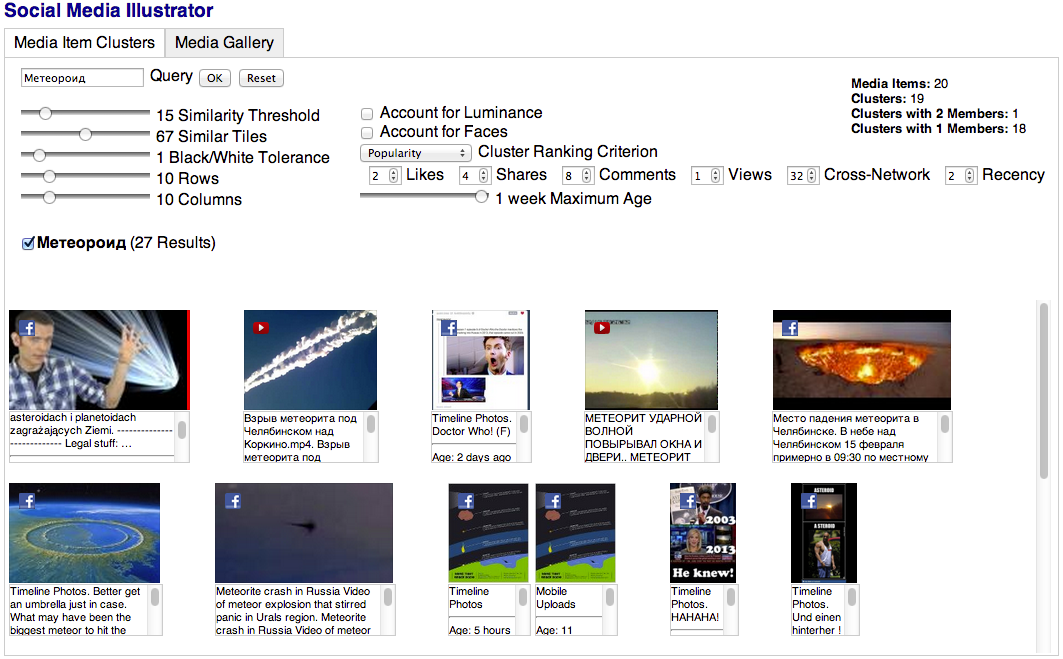
\includegraphics[width=0.57\linewidth]{./application.png}}
  \caption{Media Item Clusters tab of the Social Media Illustrator application
  with individual and clustered (bottom middle) media items from Facebook and YouTube,
  ranked by popularity for the Russian query
    \fontencoding{T2A}\selectfont Метеороид \fontencoding{T1}\selectfont}
  \label{fig:application}
\end{figure*}

\begin{figure*}[t!]
  \centering
  \setlength{\fboxsep}{1pt}
  \fcolorbox{light-gray}{white}{
  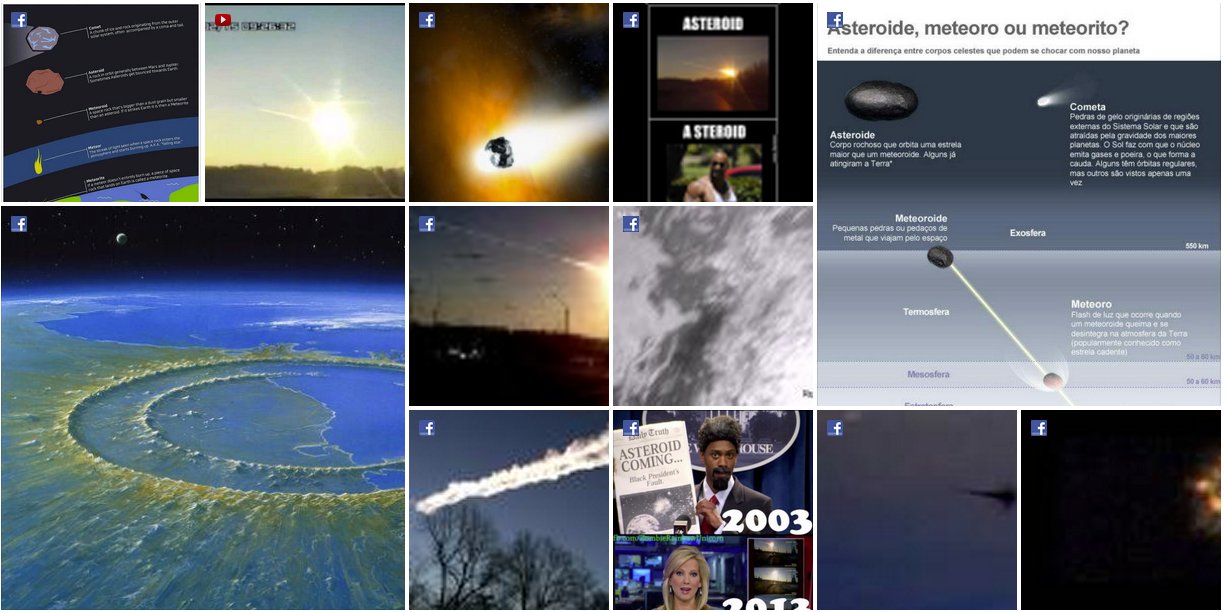
\includegraphics[width=0.57\linewidth]{./media-gallery.png}}
  \caption{Zoomed view of the Media Gallery tab of the application
    showing an automatically generated media gallery in \emph{loose order, varying size} style
    featuring ranked media items stemming from Facebook and YouTube for the query
    \fontencoding{T2A}\selectfont Метеороид \fontencoding{T1}\selectfont}
  \label{fig:media-gallery}
\end{figure*}

\bibliographystyle{abbrv}
\bibliography{www2013devtrack}

\end{document}